\chapter{Some key concepts, terms, and ways of thinking about English grammar}\label{ch:1}


\epigraph{why do we need\\
to name everything\\
\& then argue about\\
the names?}{}


\section{Introduction}\label{sec:intro1}

If the idea of teaching English grammar makes you nervous, you're not alone. Many aspiring English-language teachers feel intimidated by grammar, unsure about the difference between an adverb and an adjective, or worried they don't know enough about the intricacies of the language they hope to teach. But here's a secret: understanding grammar isn't about memorizing a set of rigid rules. There will, of course, be memorization, but that won't be of much use unless we develop new ways of thinking about language~-- ways that will help us make sense of English and, eventually, help your future students do the same.

This chapter is designed to ease you into this new way of thinking. I'm not going to start by bombarding you with entirely unfamiliar terms like \textit{clitic}, \textit{deixis}, or \textit{ergative}, and I won't be setting out any complex rules. Instead, we'll begin by questioning some basic assumptions about language and exploring how we define the things we think we understand.

We'll start with some fundamental concepts and gradually build up to more specific grammatical ideas. Along the way, we'll develop critical thinking strategies that are crucial for anyone planning to teach language. You'll learn to look for counterexamples, to consider different perspectives, and to recognize the difference between everyday and technical uses of terms.

Don't worry if you feel unsure about your grammar knowledge right now. By the end of this chapter, you'll have a basic toolkit for thinking about language that will help you approach grammar with more confidence. And we'll start with a question that might seem simple at first, but will challenge us to think more deeply: What makes soup soup?

It seems like a silly, irrelevant, and trivially easy question, at least until you try to answer it. What's the difference between tea and soup, sauce and soup, porridge and soup, stew and soup, juice and soup. Don't forget that there's gazpacho, salmorejo, cucumber soup, and other cold soups.\footnote{\href{https://youtu.be/Y1HVTNxwt7w}{A video} from BBC Scotland is the source of the soup question.}

This isn't special to soup. Most things, when you start looking at examples and counter-examples, turn out to be really hard to pin down. The problem is that we try to define things by picking out necessary and sufficient conditions.

\subsection{Necessary and Sufficient Conditions}\label{sec:conditions}

\is{definition!necessary and sufficient conditions|(}\is{necessary and sufficient conditions|(}In both philosophical and scientific circles we find the concept of ``necessary and sufficient conditions''. A necessary condition must be present for acceptance; a sufficient condition, if present, guarantees acceptance. In other words, when we say a condition is necessary and sufficient for a word to be categorized as a noun, we mean that the word cannot be a noun unless it possesses characteristic A, and that if characteristic A is present, the word is definitely a noun.

A clear and straightforward example of this is the concept of even numbers in mathematics. An integer is an even number if dividing it by two results in another integer. This is both a necessary and sufficient condition for an integer to be even. No even number exists that is not divisible by two in this way (making it a necessary condition), and any such number is always even (making it a sufficient condition).\footnote{Even something as seemingly definitive as the difference between even and odd numbers may not be as clear cut as we think \autocite{Heubner2018}.}\is{necessary and sufficient conditions|)}\is{definition!necessary and sufficient conditions|)}

So, from philosophical abstractions to mathematical certainties, necessary and sufficient conditions often frame our understanding of concepts.

\subsection{The trouble with (linguistic) definitions}\label{sec:definitions}

\is{definition!linguistic!challenges|(}But when we come to language and its components, definitions that use necessary and sufficient conditions tend to fail. Let's say you defined a \is{noun, noun phrase (NP)|(}noun as `a word that denotes a person, place or thing' and you defined a \is{verb, verb phrase (VP)|(}verb as `an action word'. Take a moment to think about what kind of word could be more of an action word than \textit{action}. And then think about whether \textit{action} is a verb or a noun (hint:\href{https://www.ldoceonline.com/}{~check a dictionary}).

To be clear, \textit{action} is usually a noun, but it's also a verb (e.g., \textit{We need to \uline{action} these tasks before the end of the day.}). Or perhaps it would be better to say that there are two \textit{action}s, the more common one being a noun and the relatively rare one being a verb.

But it's not just \textit{action}. Consider the definition of \href{https://www.ldoceonline.com/dictionary/violation}{\textit{violation}}. It's a noun, and it's an action. The same is true of many nouns, from \textit{blow} to \textit{cue} and \textit{signal} to \textit{sin}. They are defined using the phrase ``the action of\dots'', so this pretty much destroys the very common idea that a noun is a person, place, or thing and a verb is an action word. \is{noun, noun phrase (NP)!denotation}Nouns can be action words too.\is{verb, verb phrase (VP)|)}\is{noun, noun phrase (NP)|)}

We define words to understand language, but we need to understand language to define words.

\begin{tcolorbox}[float*, title=A thinking trap, colback=white]
    \is{thinking trap!confirmation bias|(}You see four cards on a table. Each card has a number on one side and a color on the other side. The sides you can see have a 3, an 8, and the colors blue and red. To check the rule ``if a card has an even number on one side, then the other side is blue,'' which card(s) should you flip over?
    \begin{center}
        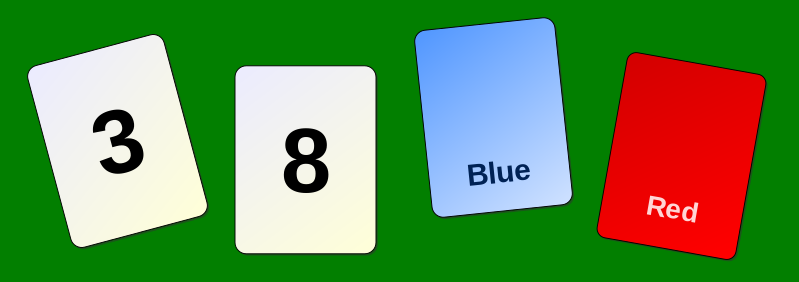
\includegraphics[width=0.5\textwidth]{figures/wason.png}
        \tiny \captionof{figure}{Image by User:Life of Riley and User:Domdomegg, CC BY-SA 4.0 \href{https://creativecommons.org/licenses/by-sa/4.0}{via Wikimedia Commons}}
    \end{center}
    Many people would say the 8 and the blue. And indeed, you need to check the 8. If the other side is not blue, the rule is violated. On the other hand, flipping the blue card doesn't test the rule. The rule says nothing about odd numbers at all, only about even numbers, which is presumably why almost nobody checks the 3 card. So, whether the other side of the blue card is an even or odd number, it doesn't affect the rule. The red holds the key. Turn it and find an even number and the rule would be violated.

    \is{counterexample}Our goal is not only to affirm the rule but also to look for counterexamples, situations where the rule fails. This is just as crucial when we contemplate the definitions of linguistic concepts. A definition that either encompasses non-members or excludes members is not a good definition. If we're assessing ``an action word'' as a proper definition for a verb, we need to consider both affirming and contradicting evidence. For example, we can check whether the word \textit{run} is an ``action word'' (it is) and whether it is a verb (it is). On the other hand, we also need to look for contradicting evidence such as words that are considered ``action words'' but are not verbs, like \textit{action} or \textit{run} in the sentence \textit{I went for a run}. Similarly, words like \textit{exist} and \textit{sense}, which are not necessarily perceived as ``action words'', can be verbs.\is{thinking trap!confirmation bias|)}
    
\end{tcolorbox}

\is{noun, noun phrase (NP)!vs verb|(}\is{verb, verb phrase (VP)!vs noun|(}But maybe we can save something here. Can you think of any words denoting physical objects that are verbs? Spend a few moments.

\bigskip

\is{noun, noun phrase (NP)!denotation}I think it's safe to say that nouns and verbs can both denote actions, but \is{verb, verb phrase (VP)!denotation}verbs never denote physical objects, or people or places, for that matter. We need a noun for that. This leads us to the following conclusion:
\begin{itemize}[noitemsep]
    \item It's true that ``persons, places, and things, are only denoted by nouns,'' but
    \item it's false that ``nouns only denote persons, places, and things.''
\end{itemize}
That's a subtle difference, but an important one. Nouns can denote a wider variety of things, while verbs are more limited, and the sets of things that nouns and verbs can denote overlap.\is{noun, noun phrase (NP)!vs verb|)}\is{verb, verb phrase (VP)!vs noun|)}

So far, we've identified three issues when it comes to defining nouns and verbs. When it comes to adjectives, and other lexical categories, similar points apply, but let's take stock right now.
\begin{enumerate}[noitemsep]
    \item A simple definition with necessary and sufficient conditions will include things that don't belong (gravy is made from stock but it's not soup) and exclude things that do belong (gazpacho is served cold but it's still soup).
    \item We can't just make our definition fit the examples we have in mind. We need to consciously think of \is{counterexample}counterexamples.
    \item Sometimes we need to restate our ideas to accurately express them.
\end{enumerate}\is{definition!linguistic!challenges|)}

As language teachers, we use categories like \textsc{noun} and \textsc{verb} a lot. But categorizing words is a tool, not the end goal. The purpose of categorizing is to be able to make general statements about the world or, in our case, about language.

And here's why this matters: If you have the wrong categories, then you'll have more ``rules'' and more ``exceptions'' than you need. Having the right categories means you can say more with less, and this makes life easier for you and for your students.

\clearpage
\begin{tcolorbox}[title=Questions, colback=white]
1. What's the main goal of this course?

2. What's wrong with the idea that an English noun is the name of a person, place, or thing?

3. Which statement is a necessary and sufficient definition of English verbs: A) verbs denote actions. B) actions are denoted by verbs. C) neither of the above.

4. How is the soup video relevant to defining word categories?

5. What is the thinking trap that we often fall into and which we should try to avoid?
\end{tcolorbox}

\begin{tcolorbox}[title=Answers, colback=white]
1. We are gaining facility with the analysis of language so that we can provide our students with the tools that they can use to decide how to speak English.

2. In English, nouns denote a far wider range of concepts than this, including actions and characteristics.

3. C) is correct. The category of verbs cannot be reliably defined based on denotations.

4. It illustrates that categories in general don't have necessary and sufficient properties.

5. We look only for confirmatory evidence to support our hypotheses, and we fail to look for evidence that might disconfirm them.
\end{tcolorbox}

\subsection{What do we mean by \textit{phrase}?}\label{sec:phrases}

\is{phrase!technical vs everyday meaning|(}Just as we found with nouns and verbs, some of our most basic assumptions about language can trip us up. Take the word \textit{phrase}, for instance. You probably think you know what it means~-- after all, we use phrases every day. In everyday language, a phrase is just a group of words that go together to express an idea, like \textit{on the table} or \textit{be going to}. And that's a perfectly good sense of \textit{phrase}. It's the most common one, and the one most people associate with the word.

But there is also a technical sense, and that's the one I'll be using throughout. \is{phrase!headed structure|(}A \textsc{phrase} in English grammar is a specific type of structure with two key properties:
\begin{enumerate}[noitemsep]
    \item It has a \is{head!in phrase structure}\textsc{head}~-- a core word that determines the basic properties of the whole phrase
    \item It may have \is{dependent}\textsc{dependents}~-- optional words or other phrases that modify or complete the meaning of the head
\end{enumerate}\is{phrase!headed structure|)}
This is quite different from the everyday notion of `words that go together'. For example, \textit{coffee and tea} might seem like a perfectly good phrase in everyday speech, but technically it's not a single phrase~-- it's a coordination of two noun phrases (\textit{coffee} and \textit{tea}) joined by \textit{and} (see Section \ref{sec:coordination} for more about coordinations). None of these words is the head of the whole expression.

Examples of phrases~-- in the everyday sense~-- that aren't phrases in the technical sense include:

\setlength{\columnsep}{0pt}
\begin{multicols}{2}
\ea
    \ea \label{ex:missing_dependents} \textit{can't help but}
    \ex \textit{let alone}
    \ex \label{ex:missing_dep_context} \textit{{\ob}want to{\cb} try again}
    \ex \textit{{\ob}pick up{\cb} the pencil}
    \ex \textit{good or bad}\label{ex:missing_head}
    \ex  \textit{salt and pepper}
\z
\z
\end{multicols}
Examples in (\ref{ex:missing_dependents} \& b) are missing dependents. Those in (\ref{ex:missing_head} \&d), are potentially full phrases, but are omit dependents in the given context. Finally, those in (\ref{ex:missing_head}) have no head.

For now, there's no need to think too hard about what a phrase is. I just want to alert you to the fact that I'm going to be using \textit{phrase} in a way that might seem familiar but is actually subtly different.\is{phrase!technical vs everyday meaning|)}

This distinction between the technical meaning of \textit{phrase} and the everyday meaning is not so unusual. Academics often adopt common words but give them a technical meaning. This doesn't mean that the everyday sense is wrong or that the technical one is; it's common for words to have various meanings. But it's useful for English teachers to be aware that many linguistic terms, like \textit{phrase}, have a technical sense which is similar to but slightly different from the everyday meaning.

This technical definition of phrases will be important throughout the following chapters. When we talk about noun phrases, verb phrases, and other types, we'll always be referring to these headed structures, whether or not they have dependents, not just any group of connected words. To be explicit, this allows for one-word phrases such as those underlined in (\ref{ex:one-word-phrases}).

\ea \label{ex:one-word-phrases}
    \ea \textit{\uline{Stop}!}
    \ex \textit{Would you like \uline{pepper} with that?}
\z\z

With this clearer understanding of what we mean by \textit{phrases}, we can now turn to the specific types of phrases we find in English, starting with noun phrases and the nouns that head them.

\section{Nouns and noun phrases}\label{sec:nouns}

%The image in Fig. \ref{fig:greeneggs} shows the relationship between all the words in \href{https://books.google.ca/books?id=h7w4DwAAQBAJ&lpg=PP1&dq=green%20eggs%20and%20ham&pg=PP1#v=onepage&q=green%20eggs%20and%20ham&f=false}{\textit{Green eggs and ham} by Dr. Seuss}. The nouns are in blue.

%\begin{figure}[h!]
%    \centering
%    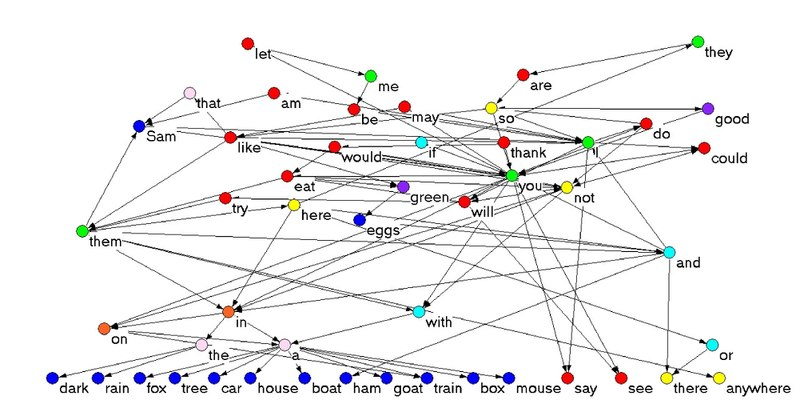
\includegraphics[width=0.9\textwidth]{figures/page1-800px-Green_Eggs_and_Ham_word_adjacency_network.pdf.jpg}
%    \caption{Network of concatenated words. Image by \href{https://commons.wikimedia.org/wiki/File:Green_Eggs_and_Ham_word_adjacency_network.pdf}{Gigas Devil}, \href{https://creativecommons.org/licenses/by-sa/4.0}{CC BY-SA 4.0}, via Wikimedia Commons.}
%    \label{fig:greeneggs}
%\end{figure}

\is{noun, noun phrase (NP)!definition challenges|(}\is{noun, noun phrase (NP)!properties of|(}There's no perfect definition of \textit{noun},\footnote{This book is about English, and so, here and throughout, I mean English nouns, verbs, tenses, etc. When I want to talk about nouns in languages in general, I'll make that clear.} just as there's no perfect definition of \textit{soup}, but we can get very close, as long as we're willing to hedge with words like \textit{can}, \textit{almost}, and \textit{typically}.

I will use words here that have not yet been explained. This may be frustrating, but it is inevitable. Syntax is a system, and its elements can only be defined in relation to each other. The meaning of the other words will become clear soon.

\begin{itemize}[noitemsep]
    \item Nouns can denote almost anything.
    \item A word that denotes a person, place, or thing is a noun \\(but not ``a noun is a word that denotes person, place, or thing'').
    \item A word that is countable is a noun \\(but not ``all nouns are countable'').
    \item Almost any word that is plural is a noun (but not ``all nouns can be plural'').
    \item Nouns often follow \textit{the} or \textit{a} (but not ``words following \textit{the} or \textit{a} are nouns'').
    \item Nouns head noun phrases (NPs).
    \item Noun phrases can typically include adjective phrases as modifiers \\(and other types of phrases typically can't).
    \item Noun phrases can't typically include adverb phrases as modifiers \\(but other types of phrases typically can).
    \item \is{noun, noun phrase (NP)!functions as subject/object}Noun phrases can perform a variety of functions, including subject and object (but not ``subjects and objects are noun phrases'').\footnote{Some examples follow, and I'll say more about what subjects and objects are later.}
    \item \is{noun, noun phrase (NP)!possessive}Noun phrases can typically be possessive.\footnote{\textit{The Cambridge grammar of the English language} uses the term \textsc{genitive} instead of possessive because the relationship is often not one of possession. The term \textsc{possessive}, though is much more common, so I will use it here, as long as you promise to remember that \textit{your pet's vet} is not a vet possessed by your pet.}
\end{itemize}\is{noun, noun phrase (NP)!properties of|)}\is{noun, noun phrase (NP)!definition challenges|)}

Importantly, each of these characteristics can be odd or unfamiliar to English-language learners. In the other languages they speak, there may be no plural nouns, for example. So the elements of the definition point to facts about English nouns that may be useful for English-language learners to learn. It's also important to note that many of the statements are not commutative (multiplication is commutative but division isn't; $X \times Y = Y \times X$ but $X \div Y \neq Y \div X$). In other words, the way you say something can be really important. 

Unfortunately, people often won't notice~-- or will later disregard~-- the difference between ``nouns can typically follow \textit{the} or \textit{a}'' and ``a word that follows \textit{the} or \textit{a} is typically a noun.'' In fact \textit{the} is followed immediately by a noun about 34,500 times per million words, while it's followed by a non-noun about 48,400 times per million words.\footnote{Counts are from the Corpus of Contemporary English \citep{COCA}.} So, while the next word after \textit{the} is often a noun, anyone relying on this to be true will be wrong more often than they're right.

\subsection{Some examples}\label{sec:examples}
The following is meant to make the characteristics listed above more concrete by providing examples. After considering each set of examples, try to think of nouns that do NOT have one or more of the properties listed. In other words, look for counter-examples.


\paragraph*{What nouns denote}
\is{noun, noun phrase (NP)!denotation}We've already seen how nouns can denote actions. We also have characteristics (e.g., \textit{beauty}, \textit{happiness}, \textit{size}, \textit{aptitude}), states (e.g., \textit{absence}), relations (e.g., \textit{togetherness}, \textit{superiority}), and on and on.

\paragraph*{Countability}

\is{countability (count vs non-count nouns)|(}Here are some examples of count nouns: \textit{apple}, \textit{book}, \textit{chair}, \textit{pen}, \textit{tree}, \textit{giraffe}, \textit{telescope}, \textit{flute}, \textit{cathedral}, \textit{quasar}, \textit{enzyme}. And here are some non-count nouns: \textit{water}, \textit{information}, \textit{rice}, \textit{music}, \textit{furniture}, \textit{advice}, \textit{syrup}, \textit{flour}, \textit{machinery}, \textit{courage}, \textit{syntax}, \textit{kinship}.

\paragraph*{Plural nouns}
\is{noun, noun phrase (NP)!plural forms}Consider the following examples of plural nouns: \textit{we}, \textit{women}, \textit{children}, \textit{students}, \textit{things}, \textit{eyes}, \textit{police}, \textit{fish}, \textit{words}, \textit{thanks}, \textit{feet}, and \textit{problems}.

\paragraph*{Nouns following \textit{the} or \textit{a}}
These examples are very simple noun phrases with \textit{the} and \textit{a} plus a head noun: \textit{the world}, \textit{a lot}, \textit{the way}, \textit{the end}, \textit{the people}, \textit{a man}, \textit{the day}, \textit{a couple}, and \textit{a year}.

\paragraph*{Noun phrases with adjective-phrase modifiers and head nouns}
\is{modifier!adjective phrase in NP}Next, examine these noun phrases with adjective-phrase modifiers and head nouns. The adjective phrase is underlined, and the head noun is double-underlined: \textit{a \uline{long} \uuline{time}}, \textit{a \uline{little} \uuline{bit}}, \textit{\uline{other} \uuline{people}}, \textit{the \uline{twelfth} \uuline{one}}, \textit{the \uline{supreme} \uuline{court}}, \textit{a \uline{very good} \uuline{morning}}, \textit{the \uline{only} \uuline{way} I know}, \textit{an \uline{old} \uuline{man}}, and \textit{\uline{social} \uuline{media}}.

\paragraph*{Noun phrases functioning as subjects}
\is{subject}In each of the following sentences, the underlined noun phrase is the subject: \textit{\uline{you} win}; \textit{\uline{time} is on my side}; \textit{\uline{a little bit} goes a long way}; \textit{\uline{other people} can help}; \textit{\uline{the supreme court} released its decision}; \textit{often, \uline{the twelfth one} is perfect}; \textit{\uline{a very good morning} is a rare pleasure}; \textit{on Monday, \uline{the shop} will be closed}; and \textit{what does \uline{human rights} mean}.


\paragraph*{Possessive noun phrases}
\is{noun, noun phrase (NP)!possessive}The following noun phrases are possessive: \textit{my}, \textit{mine}, \textit{its}, \textit{whose}, \textit{Brett's}, \textit{time's}, \textit{other people's}, \textit{the supreme court's}, and \textit{the lady who lives here's}.

\paragraph*{``Good'' examples of nouns}
A word like \textit{school}, for instance, has all the properties listed above. It's a prototypical noun, a ``good'' example. Here are some other generally good examples of nouns, though they might not each exhibit every property given above: \textit{person}, \textit{way}, \textit{day}, \textit{life}, \textit{man}, \textit{school}, \textit{student}, \textit{thing}, \textit{house}, \textit{family}, \textit{work}, \textit{part}, \textit{night}, \textit{country}, \textit{government}, \textit{place}, \textit{money}, \textit{water}, and \textit{room}. Which nouns lack which properties?

\paragraph*{``Less good'' examples of nouns}
A word like \textit{umbrage}, for instance, is missing a number of the properties listed above. For instance, it has no plural, nor do you find possessive NPs with \textit{umbrage} as the head. It doesn't denote a physical object, a person, or a place. It is not countable and therefore it doesn't follow \textit{an}. It has other oddities too; can you think of any?

Other not-so-good examples include: \textit{contemplation}, \textit{crockery}, \textit{furniture}, \textit{sake} (as in \textit{for heaven's sake}), \textit{shrift}, \textit{what}, and \textit{behalf}. What properties to each of them lack? Practice thinking of nouns that are missing one or more of the properties. Use a good dictionary to check if you're not sure the word is a noun.\footnote{I would suggest the \href{https://simple.wiktionary.org/wiki/Main_Page}{\textit{Simple English Wiktionary}}. I'm an editor there, and I'll stand behind the category system there. If you don't find the word you're looking for there, then try the \href{https://www.ldoceonline.com/}{\textit{Longman Dictionary of Contemporary English}}.}\is{countability (count vs non-count nouns)|)}


\begin{tcolorbox}[title=Questions, colback=white]
From each group of statements, choose the one that is true and relevant.\footnote{\rotatebox{180}{
    \begin{minipage}[t]{0.9\linewidth}1. a; 2. a; 3. c; 4. b; 5. a; 6. c
    \end{minipage}
    }
}
    \begin{enumerate}[noitemsep]
        \item\begin{enumerate}[noitemsep]
            \item Nouns can denote almost anything from objects to actions to characteristics.
            \item A noun is a word that denotes only people, places, and things.
        \end{enumerate}
        \item\begin{enumerate}[noitemsep]
            \item Any word that is countable is a noun.
            \item You can count nouns.
            \item All nouns are countable.
        \end{enumerate}
        \item\begin{enumerate}[noitemsep]
            \item A plural noun always ends in an \textit{-s}.
            \item Any noun can be plural.
            \item Almost any word that is plural is a noun.
        \end{enumerate}
        \item\begin{enumerate}[noitemsep]
            \item A noun is any word that follows \textit{the} or \textit{a}.
            \item Nouns can typically follow \textit{the} or \textit{a}.
            \item Any word that typically follows \textit{the} or \textit{a} is a noun.
        \end{enumerate}
        \item\begin{enumerate}[noitemsep]
            \item A noun phrase can typically include an adjective phrase its a modifier.
            \item A noun phrase can typically include an adverb phrase as its modifier.
            \item Any phrase with an adjective phrase as its modifier is a noun phrase.
        \end{enumerate}
        \item\begin{enumerate}[noitemsep]
            \item Nouns themselves can perform a variety of functions, including subject and object.
            \item Noun phrases function only as subject or objects.
            \item Noun phrases can perform a variety of functions, including subject and object.
        \end{enumerate}
    \end{enumerate}
\end{tcolorbox}



\begin{tcolorbox}[title=Find the nouns, colback=white]
    In reality, from the top of the ladder, standing erect on the last rung, you could just touch the Moon if you held your arms up. We had taken the measurements carefully (we didn't yet suspect that she was moving away from us); the only thing you had to be very careful about was where you put your hands. I always chose a scale that seemed fast (we climbed up in groups of five or six at a time), then I would cling first with one hand, then with both, and immediately I would feel ladder and boat drifting away from below me, and the motion of the Moon would tear me from the Earth's attraction. Yes, the Moon was so strong that she pulled you up; you realized this the moment you passed from one to the other: you had to swing up abruptly, with a kind of somersault, grabbing the scales, throwing your legs over your head, until your feet were on the Moon's surface.\footnote{\rotatebox{180}{
    \begin{minipage}[t]{0.9\linewidth}
        \textit{reality}, \textit{top}, \textit{ladder}, \textit{rung}, \textit{you}, \textit{Moon}, \textit{you}, \textit{your}, \textit{arms}. \textit{We}, \textit{measurements}, \textit{we}, \textit{she}, \textit{us}; \textit{thing}, \textit{you}, \textit{you}, \textit{your}, \textit{hands}. \textit{I}, \textit{scale}, \textit{we}, \textit{groups}, \textit{time}, \textit{I}, \textit{ladder}, \textit{boat}, \textit{me}, \textit{motion}, \textit{Moon}, \textit{me}, \textit{Earth's}, \textit{attraction}. \textit{Moon}, \textit{she}, \textit{you}; \textit{you}, \textit{moment}, \textit{you}, \textit{other}; \textit{you}, \textit{kind}, \textit{somersault}, \textit{scales}, \textit{your}, \textit{legs}, \textit{your}, \textit{head}, \textit{your}, \textit{feet}, \textit{Moon's}, \textit{surface}.
    \end{minipage}
    }
}\\\phantom{~}\hfill~-- Italo \citeauthor{calvino2018}, ``The distance of the moon''

\end{tcolorbox}

\subsection{Number: Countability, singularity, and plurality}\label{sec:count}

\is{countability (count vs non-count nouns)|(}\is{number|(}Countability is a remarkably easy concept. If you can say ``two $x$'', where $x$ is the noun, then $x$ is a count noun. For example, \textit{two pencils} is fine so \textit{pencil} is a count noun. But you can't say *\textit{There are two furnitures} (* means it's ungrammatical), so \textit{furniture} is a non-count noun. Sometimes, words like \textit{jeans} seem like they might be count nouns, but it turns out that we count \uline{pairs} of jeans, not jeans. Another perhaps-surprising example of a non-count noun is \textit{police}: we don't say *\textit{two police were standing on the corner}. Instead, we say \textit{two} (\textit{police}) \textit{officers}, where \textit{officer} is a count noun. \textit{Meat} is an example of a noun that is not usually countable but can be if we mean `kinds of meat'. This way of creating count nouns from non-count nouns in a `kinds-of' meaning is quite common.

The concept of countabiliy may be easy to understand, but the trick is in knowing for which nouns one can or cannot say ``two $x$''. It may seem quite obvious to you what is countable and what is not, and you might think that because it's so obviously, it will be very easy to explain to students. You might even have some deep down feeling that somebody who failed to get the concept must be a little slow. But if you have that feeling, it's only because you already know. In fact, even experts can have a very muddled concept of countability. Take, for example, the \textit{Longman Dictionary of Contemporary English}.

\is{thinking trap}I check this excellent dictionary regularly because it has very informative entries, but if you look up \href{https://www.ldoceonline.com/dictionary/uncountable/}{\textit{uncountable}}, you'll find the following definition:

\begin{quote}
    An uncountable noun has no plural form and refers to something which cannot be counted or regarded as either singular or plural, for example `money' or `happiness'.
\end{quote}
Sadly, Longman has fallen into the very thinking trap we considered earlier: They thought up a few matching examples and failed to consider counter examples. Let's look, on their behalf, for the counter examples. Can you think of a noun that \uline{does} have a plural form but which \uline{cannot} be counted, in other words, a plural noun for which you can't say ``two $x$''? We've already considered at least one example in Section \ref{sec:examples}. See the footnote after you've given it some thought.\footnote{\rotatebox{180}{
    \begin{minipage}[t]{0.9\linewidth}
        \is{plural!plural-only nouns}We've already seen \textit{police}. \textit{Pants} is another example. We say \textit{two pairs of pants}, not *\textit{two pants}. Still others include \textit{groceries}, \textit{remains}, \textit{clothes}, \textit{scissors}, \textit{gentials}.
    \end{minipage}
    }
} The funny thing is that the dictionary applies these labels correctly to individual words. The entry for \href{https://www.ldoceonline.com/dictionary/glasses/}{\textit{glasses}}, for instance, is correctly labeled as \textsc{uncountable}. The editors know that \textit{glasses} is plural and that it's a non-count noun, but they haven't noticed that their definition is in conflict with their practice.



\begin{tcolorbox}[title=Why does this matter?, colback=white]
    Consider the following: 
    
    \ea
        \ea[]{\textit{I had }(\textit{a})\textit{ tea.}}\label{ex:tea}
        \ex[]{\textit{I had a cookie.}}\label{ex:cookiea}
        \ex[*]{\textit{I had cookie.}}\label{ex:cookie}
        \z\label{ex:blank}
    \z
    
    \is{countability (count vs non-count nouns)!and determiners}\is{determiner!and countability}\is{determiner!and singular count nouns}I hope you'll agree with me that (\ref{ex:tea}) is perfectly fine with or without the \textit{a}, but that in (\ref{ex:cookiea}) the \textit{a} is required and that (\ref{ex:cookie}) is ungrammatical. What could explain this difference? It turns out that singular count nouns require a determiner~-- a term I'll explain in a later chapter. The words \textit{a} and \textit{the} can function as determiners. So can words like \textit{one}, \textit{his}, \textit{Brett's}, \textit{every}, etc. So, if you have a concept of count vs. non-count, and you've got a sense of singular vs. plural, you can use that to explain why (\ref{ex:tea}) is fine either way, but (\ref{ex:cookie}) isn't. This is what I mean when I say that we're working with a system: as you learn about some parts of it, you can use those parts to solve mysteries in other areas that are not obviously connected.
\end{tcolorbox}

So, we see that the definition of \textit{uncountable} in the Longman dictionary is wrong, even though it's generally a very good dictionary and even though its own entry for \textit{glasses} (among many others) contradicts its definition of \textit{uncountable}. Maybe this determination isn't so easy. But even if creating a good definition turns out to be a little harder than we thought, it may still feel like it should be quite obvious what is countable and uncountable based on certain properties. If that were the case, though, then we would find that singular nouns always translated as singulars and plural nouns always as plurals (at least, when a language has plurals). \is{countability (count vs non-count nouns)!cross-linguistic variation|(}But in the realm of countability, what counts in one language may not count in another.

If you're multilingual, perhaps you've already run into this. Can you think of any counterexamples?\footnote{Pairoj Kunanupatham reminded me.}
In each numbered example below, the first line is the example in another language, the second is a word-for-word gloss, and the third is the natural English translation. In some second lines, you'll see -\textsc{pl}, which means `this is plural'. (In other languages, being plural is common not just for nouns but for other words too.)

\ea
\ea[]{\gll \textit{J'} \textit{ai} \textit{coupé} \textit{mes} \uline{\textit{cheveux}}.\\
     I have cut my-\textsc{pl} hairs-\textsc{pl}.\\
    \glt `I cut my hair.'}\label{ex:cheveaux}
\ex[]{\gll \uline{\textit{Картошка}} \textit{была} \textit{вкусной}.\\
    potato is hot\\
    \glt `The potatoes are hot.'}\label{ex:Картошка}
\ex[]{\gll\textit{ekṭa} \uline{\textit{khobor}} \textit{āche}\\
    a news is/exists\\
    \glt `There's some news.'}\label{ex:khobor}
\ex[]{\gll\textit{Þe} \uline{\textit{pease}} \textit{wæs} \textit{swete}.\\
    the pea was delicious\\
    \glt `The peas were delicious.'}\label{ex:pease}
\z
\z
\is{number!cross-linguistic variation}In \refp{ex:cheveaux}, the French word \textit{cheveux} is a plural count noun  (though it would be rare to count hairs, even in French), while in English it's usually a singular non-count noun. To some extent, this is motivated by the fact that it would be impractical to count the hairs you cut, but, as the French shows, there's no need to enumerate them; you could just say \textit{I cut my hairs} and leave it at that. To some extent, the English way of thinking of hair as uncountable comes from it behaving somewhat like a single mass. But again, as the French shows, there are other ways to think about it.

The Russian word \textit{kартошка} `potato' in \refp{ex:Картошка}, is non-count singular. Of course, English also has a non-count singular sense of \textit{potato} as in \textit{You dropped some potato on the floor}, but, in my Ontario dialect at least, \textit{mashed potatoes} is plural, regardless of the number of potatoes that were mashed. In contrast, Russians would use the singular where Ontarians might be momentarily confused if you asked them to pass the potato, thinking you were asking for an intact tuber.

In the Bangla example (\ref{ex:khobor}), \textit{khobor} `news' is a count noun, while in English \textit{news} is strictly non-count. While English requires phrases like \textit{piece of news} or \textit{news item}, Bangla speakers directly count \textit{khobor}. To some extent, this reflects a different way of conceptualizing information~-- as discrete pieces rather than a continuous mass. But as the English phrase \textit{piece of news} shows, we can think about it either way. It's just that Bangla chooses one perspective while English picks the other.

\is{plural!foreign plurals}Finally, \refp{ex:pease} is Middle English. The Modern English word \textit{pea} comes from a mistaken singular; the word was \textit{pease}, which ends with the same \textipa{/z/} sound we find at the end of many plurals such as \textit{bees} or \textit{peas}. But it wasn't a plural. It was just part of the word, like the \textipa{/z/} at the end of \textit{ease} or \textit{jazz}. Still, somewhere along the way, some folks started to think about peas in the way they think about pebbles instead of the way they think about wheat or corn. And so it got reanalyzed as a plural, and \textit{pease} became \textit{peas}. This shows you that even speakers of the same language can think differently about words for the same stuff.

This peculiarity isn't limited to historical changes. Think about how English treats closely related food items: *\textit{wheats} is ungrammatical and \textit{wheat} is strictly non-count, yet we have both \textit{oat} and \textit{oats}, though \textit{oat} is only marginally countable. Then there's \textit{peas}, which can function in all these ways.

What makes the point even clearer is that synonyms in English aren't even consistently count or non-count. For example, \textit{advice} is a non-count noun, but \textit{opinion} is a count noun, even though, when we give advice, usually it's our opinions we're giving. Can you think of any other pairs like this?

Each has a synonym that, at least in the relevant sense, is uncountable: \textit{story}, \textit{idea}, \textit{hole}, \textit{song}, \textit{nap}, \textit{lies}. See the footnote after you've given it some thought.\footnote{\rotatebox{180}{
    \begin{minipage}[t]{.9\linewidth}
        \textit{story} \& \textit{fiction}, \textit{idea} \& \textit{knowledge}, \textit{hole} \& \textit{space}, \textit{song} \& \textit{music}, \textit{nap} \& \textit{sleep}, \textit{lies} \& \textit{bullshit}.
    \end{minipage}
    }
} \is{countability (count vs non-count nouns)!cross-linguistic variation|)}

It's easy to think that ideas that we take for granted, such as whether something is countable or not, are objective facts. In many cases like this, they are actually inter-subjective judgments, many entirely unpredictable to those outside the community of speakers of a given language or dialect.

And yet, many language-teaching materials treat countability as if it were obvious from mere introspection. Far from it! Consider the following explanation from \citet{allen2008}, a textbook for children. It's perfectly simple if you speak English and almost entirely unhelpful if you don't.

\begin{quote}
    You can see from the list that some nouns can be counted and others can not. For example, if you want to tell your friend about the fruit on the tree, you could tell them your tree has plenty of plums on it. The noun `plum' is countable so you have to make it plural by adding an `-s-' (sic). Or you could tell them your tree has plenty of fruit on it. In this case, the noun `fruit' is uncountable, so you can not count an `-s'. \citet[1]{allen2008}
\end{quote}

The book assumes that plums are countable because you can count them, and you can count them because they're countable. What could be easier? What about \textit{rice} and \textit{seed}? There is no way for a learner of English to guess that you can say \textit{two seeds} but not *\textit{two rices} if you mean `two grains of rice'. \textit{Two rices} can only mean `two kinds of rice', not `two grains'.

The unpredictability goes beyond nouns themselves. Remember how I said that certain words like \textit{a} and \textit{the} can function as determiners? Well, the relationship between determiners and nouns isn't as neat as you might expect. Take \textit{oats}, for instance. Despite its plural form, it often pairs better with \textit{much} as a determiner than with \textit{many}. And while \textit{an oat} is grammatically possible, it sounds odd to most speakers. Even the supposed clear distinction between \textit{less} (for non-count nouns) and \textit{few} (for count nouns) often breaks down in everyday usage. Once again, we see that what seems ``natural'' to English speakers is anything but obvious to learners~-- or indeed to someone thinking critically about the language.

There is great diversity in the world. It is important for us not be so blinded by our own intuitions as to believe that our way of categorizing stuff into that which can be counted and that which cannot is in any way natural or objective. And remember that when your students make the Standard English choice, you should respect them for having achieved an insight into the peculiar way of looking at the world shared by English speakers.\is{countability (count vs non-count nouns)|)}

\subsubsection*{What does \textit{plural} mean?} \label{sec:plural-meaning}

\is{number!singular vs plural|(}\is{plural!meaning ('not singular')|(}\is{singular!meaning ('exactly one')|(}Surely, something as basic as the distinction between singular and plural nouns would be straightforward. In English, regular plural nouns are marked with an -(\textit{e})\textit{s} (e.g., \textit{cats}, \textit{things}, \textit{students}, \textit{studies}, etc.). But what is the meaning of \textit{plural}? Most people take the everyday meaning, `consisting of or containing more than one of something.' But is this true of plural English nouns?\footnote{\citet{hauser2009} raises this point, but comes to a slightly different answer than I do.}

If it occurred to you to try to disconfirm the claim by looking for counter-examples, then you might avoid the thinking trap. So, think of some numbers that are not more than one, pair them with a variety of nouns, and see what happens. Are plural nouns grammatical in combination with these numbers? The examples in (\ref{ex:defined}) are illustrative. (In (c), $|x|$ denotes the absolute value of $x$, disregarding its sign.)

\ea \label{ex:defined}
    \ea[*]{\textit{one cats}/\textit{things}/\textit{students}/\textit{studies}/\textit{women}/\textit{mice}\hfill [definition works]}
    \ex[*]{\textit{minus one degrees}/\textit{points}/\textit{months}\hfill [definition works]}
    \ex[]{\textit{minus two degrees}/\textit{points}/\textit{months}\hfill [unclear: $-2 < 1$ but $|-2| > 1$]}
    \ex[]{\textit{zero degrees}/\textit{points}/\textit{months}\hfill [definition fails]}\is{plural!and zero}
    \ex[]{\textit{0.5 degrees}/\textit{points}/\textit{months}\hfill [definition fails]}
    \ex[]{\textit{1.0 degrees}/\textit{points}/\textit{months}\hfill [definition fails]}
    \z
\z

It seems, then, \textit{plural} does not mean `more than one'. What are we to make of this? What does seem to be true is that \textit{singular} means `exactly one (or minus one)', and so perhaps \textit{plural} means simply `not singular', which is to say `neither one nor minus one', at least as a technical term applied to English grammar. When it comes to the everyday meaning of \textit{plural}, it certainly seems to mean `more than one'. For example, nobody would agree that a bachelor has had ``plural'' marriages because he has had zero marriages. It may also be the case that plural means `more than one' in the grammar of some other language. For English at least, though, it does not mean that.

There is another case to consider, that of \textit{no}, as in (\ref{ex:no}).

\ea \label{ex:no}
    \ea[]{\textit{no way}/\textit{idea}/\textit{problem}}\label{ex:sing-no}
    \ex[]{\textit{no ways}/\textit{ideas}/\textit{problems}}\label{ex:plur-no}
    \z 
\z
The meaning of \textit{plural} in (\ref{ex:plur-no}) still seems to be `neither one nor minus one', but in (\ref{ex:sing-no}), the meaning does not appear to be `one' even though the nouns are singular. Some history of the word \textit{no} might help to explain this seeming paradox: \textit{no} is a shortening of \textit{none}, which itself comes from Old English \textit{ne} `not' + \textit{an} `one' (see also Section \ref{sec:meaning-of-negatives}). This accounts for the results in (\ref{ex:sing-no}). Over time, \textit{no} has come to also mean `not any', and this accounts for (\ref{ex:plur-no}).

Even so, perhaps it might be best to say the \strong{main} meaning of singular is `exactly one', acknowledging that neither words (e.g., \textit{one}) nor grammatical systems (e.g., the system of number) have to have a single meaning (see Section \ref{sec:fallacy-of-monosemy}).\footnote{It would be nice to have distinct terms for semantic number and syntactic number, but we seem to be stuck with \textit{singular} and \textit{plural} for both systems. See, though, Sections \ref{sec:terminology} \& \ref{box:terminology-hygiene}).}

I almost forgot about non-count nouns.\footnote{Pairoj Kunanupatham reminded me.} Consider the singular non-count nouns in (\ref{ex:sing-non-count}) and the plurals in (\ref{ex:plur-non-count}).

\ea \label{ex:undefined}
    \ea[*]{\textit{one furniture}/\textit{pottery}/\textit{footwear}\hfill [undefined]}\label{ex:sing-non-count}
    \ex[*]{\textit{one jeans}/\textit{glasses}/\textit{police}\hfill [undefined]}\label{ex:plur-non-count}
    \z 
\z
Here, the test doesn't help, not because of any mismatch between \textit{one} and the number of the noun, but because the nouns don't allow counting. The results are undefined, like dividing by zero. Semantically, though, could we argue that \textit{furniture}, \textit{pottery}, and \textit{footwear} in (\ref{ex:sing-non-count}), by virtue of being singular, denote one of something? I think we could: each denotes one class of items, and only by extension the items themselves.

What about (\ref{ex:plur-non-count})? Well, a pair of glasses is not one glass, and a group of police is not one officer, so I think the definition of \textit{plural} works, even here. 

But if you think I've loaded the dice with my explanations (you might call them ``justifications''), I take your point. Even so, the \strong{main} meaning of \textit{singular} remains `exactly one'.\is{singular!meaning ('exactly one')|)}\is{plural!meaning ('not singular')|)}\is{number!singular vs plural|)}\is{number|)}

\begin{tcolorbox}[title=Practice, colback=white]
    For each item, decide whether the noun is singular or plural and whether it is a countable sense of the noun or a non-countable sense.\\
    E.g., \textit{The two fish escaped.} countable, plural
    
    \begin{enumerate}[noitemsep]
        \item \textit{The data were accurate.}
        \item \textit{The data was accurate.}
        \item \textit{The Canadian media are generally reliable.}
        \item \textit{The Canadian media is generally reliable.}
        \item \textit{The sheep are grazing.}
        \item \textit{Little difference could be seen.}
        \item \textit{A run will be calming.}
        \item \textit{a little sugar}
        \item \textit{made of rock}
        \item \textit{The remains are buried here.}
        \item \textit{More suction, please.}
        \item \textit{Pizza is tasty.}
        \item \textit{Eating lamb is less common here.}
        \item \textit{two or three times}
        \item \textit{The children are studying.}
        \item \textit{A little knowledge can be dangerous.}
        \item \textit{the police}
        \item \textit{some new jeans}
        \item \textit{two coffees}
        \item \textit{new employment statistics}
        \item \textit{a little time}
    \end{enumerate}
\end{tcolorbox}

\newpage
\section{Glossary of Key Terms, part 1}
\begin{description}
   
   \item[counterexample] An example that disproves a proposed rule or definition, being a case where the rule fails. Good for testing linguistic definitions. See Section \ref{sec:intro1}.
   
   \item[dependent] A phrase that depends on the head. For example, \textit{the} is a dependent in \textit{the cake}. See Section \ref{sec:phrases}.
   
   \item[determiner] A dependent in a noun phrase that marks it as definite or indefinite (e.g., \textit{\uline{a} pen}, \textit{\uline{the} pen}, \textit{\uline{much more} air}, \textit{\uline{almost ten} pens}, \textit{\uline{my} pen}). See Section \ref{sec:count}.
   
   \item[head] The central word in a phrase that defines the phrase's type and core meaning. For example, \textit{cake} is the head noun in the noun phrase (NP) \textit{the chocolate cake}.  See Section \ref{sec:phrases}.
   
   \item[necessary condition] One that must be present for membership in a category. For example, having a head is a necessary condition for being a human, and having a head is a necessary condition for being a phrase. See Section \ref{sec:conditions}.
   
   \item[noun] A word that can head a noun phrase and typically denotes entities, actions, states, or concepts. Can usually be singular or plural, though some, like \textit{furniture}, are only singular and some, like \textit{proceeds}, plural only. See Section \ref{sec:nouns}.

       \item[noun, count] A count noun is one that can be counted (e.g., \textit{1 book}, \textit{2 ideas}). See Section \ref{sec:count}.
   
   \item[noun, non-count] A non-count noun is one that cannot be counted (e.g., *\textit{1 furniture}, *\textit{2 groceries}). See Section \ref{sec:count}.
   
   \item[phrase] (Technical) A grammatical structure consisting of a head word and any optional dependents. The head determines the phrase's core properties. See Section \ref{sec:phrases}.
   
   \item[plural] (technical) Indicating `neither one nor minus one'. See Section \ref{sec:count}.
   
   \item[singular] Denoting exactly one of something (or in some cases, $-1$). See Section \ref{sec:count}.
   
   \item[sufficient condition] One that, if present, guarantees membership in a category. For example, being a square is a sufficient condition for being a rectangle, and being an NP is a sufficient condition for being a phrase. See Section \ref{sec:conditions}.
\end{description}

\begin{tcolorbox}[title=Short Answer Quiz, colback=white]

Instructions: Answer the following questions in 2--3 sentences each.

[Questions 1-10 listed]
    
\end{tcolorbox}

\begin{tcolorbox}[title=Answer Key, colback=white, colframe=black, coltitle=black, fonttitle=\bfseries, colbacktitle=gray!10!white]

[Answers 1-10 listed]

\end{tcolorbox}

\clearpage
\section{Verbs and verb phrases}\label{sec:verbs}

\is{verb, verb phrase (VP)|(}So, what can we say about English verbs? Here's a list of verbs, nice verby verbs, really typical ones: 
\ea 
    \textit{jump}, \textit{walk}, \textit{ask}, \textit{turn}, \textit{work}, \textit{move}, \textit{play}, \textit{pull}, \textit{reach}, \textit{laugh} \label{ex:verblist}
\z
\is{verb, verb phrase (VP)!vs noun|(}\is{noun, noun phrase (NP)!vs verb|(}Are they action words? Of course they are. Did you notice that this could be a list of nouns though?
\begin{itemize}[noitemsep]
    \item \textit{She missed the \uline{jump}.}
    \item \textit{I went for a \uline{walk}.}
    \item \textit{That's a pretty big \uline{ask}.}
    \item \textit{Give it a \uline{turn} and see.}
    \item \textit{I went to \uline{work}.}
\end{itemize}
Each of the underlined words above is a noun. (If you doubt me, consider the characteristics we studied earlier.) But in the following cases, they're verbs.

\begin{itemize}[noitemsep]
    \item \textit{She \uline{jumped} the gap.}
    \item \textit{I \uline{walk} the dog each morning.}
    \item \textit{He's \uline{asking} for a \$10,000 raise.}
    \item \textit{It's hard to \uline{turn} the knob.}
    \item \textit{I \uline{work} in Toronto.}
\end{itemize}
So, how can we tell the difference between nouns and verbs? Sometimes we can't until they're in context. In form, they may be the same. In function, they are worlds apart. The list in \refp{ex:verblist} is perfectly ambiguous.\is{verb, verb phrase (VP)!vs noun|)}\is{noun, noun phrase (NP)!vs verb|)} Nevertheless, verbs generally have the following properties (examples below):

\begin{itemize}[noitemsep]
    \item \is{verb, verb phrase (VP)!denotation}Verbs typically denote actions and states, and they don't denote physical objects.
    \item \is{verb, verb phrase (VP)!forms (-s, -ing, past)|(}A word that has a past-tense form is a verb (but not all verbs have past-tense forms).
    \item Almost every verb has an \textit{--s} form (but not all).
    \item Almost every verb has an \textit{--ing} form (but not all).
    \item Almost every verb can follow the infinitive marker \textit{to}.\is{verb, verb phrase (VP)!forms (-s, -ing, past)|)}
    \item A verb cannot be modified by an adjective phrase.
    \item \is{verb, verb phrase (VP)!modified by adverb phrases}A verb can typically be modified by an adverb phrase.
    \item A verb phrase must be headed by a verb (always).
    \item \is{verb, verb phrase (VP)!head clauses}\is{clause!headed by verb phrase}A clause must be headed by a verb phrase (always).
    \item \is{agreement!subject-verb}A verb is often in an agreement relationship with a phrase functioning as the subject of the clause.
\end{itemize}

Let's look at some examples.

\paragraph*{What do verbs denote}
\is{verb, verb phrase (VP)!denotation}These are just everyday classifications, not technical ones, and other types could be added to the list.\\

\begin{tabular}{@{} l l}
    Actions: & \textit{come}, \textit{go}, \textit{wave}, \textit{run}, \textit{swim}, \textit{play}, \textit{hit} \\
    Mental activities: & \textit{consider}, \textit{wonder}, \textit{decide}, \textit{recall} \\
    States: & \textit{be}, \textit{seem}, \textit{own}, \textit{need}, \textit{taste}, \textit{matter}, \textit{appear}, \textit{exist} \\
    Mental states: & \textit{believe}, \textit{know}, \textit{agree}, \textit{mind}, \textit{like} \\
    Accomplishments: & \textit{win}, \textit{sleep}, \textit{become}, \textit{remain}, \textit{relax}, \textit{stop}, \textit{fail}
\end{tabular}\\

\paragraph*{Past-tense forms}\label{sec:past-forms}
\is{verb, verb phrase (VP)!forms (-s, -ing, past)}Verbs almost always have a past-tense form, while nouns never do. (Can you think of any verbs that lack a past-tense form?\footnote{\rotatebox{180}{
    \begin{minipage}[t]{0.9\linewidth}
        \is{defective verb}\textit{Must}, \textit{beware}, and \textit{ought} are the only verbs that don't have a past-tense form, as far as I know. Verbs that lack one or more forms are said to be \textsc{defective}.
    \end{minipage}
    }
})\\

Verbs:~~
\begin{tabular}{@{} l l l l l l l}
\textit{want} & $\rightarrow$ & \textit{wanted} && \textit{play} & $\rightarrow$ & \textit{played} \\
\textit{go} & $\rightarrow$ & \textit{went} && \textit{come} & $\rightarrow$ & \textit{came} \\
\textit{run} & $\rightarrow$ & \textit{ran} && \textit{make} & $\rightarrow$ & \textit{made} \\
\textit{is} & $\rightarrow$ & \textit{was} && \textit{are} & $\rightarrow$ & \textit{were} \\
\end{tabular}\\

Nouns:~
\begin{tabular}{@{} l l l l l l l}
\textit{magazine} & $\rightarrow$ & n/a && \textit{jeans} & $\rightarrow$ & n/a \\
\textit{idea} & $\rightarrow$ & n/a && \textit{government} & $\rightarrow$ & n/a \\
\end{tabular}\\
\is{word family}There are a lot of nouns and verbs that share a history, spelling, and pronunciation, such as those in \refp{ex:verblist}. They belong to the same \href{sec:family-lemma-shape-token}{word family}, but they are distinct words, in the same way that my brothers and I belong to the same Reynolds family but are, nevertheless, distinct people.



\paragraph*{Other verb forms}
\is{verb, verb phrase (VP)!forms (-s, -ing, past)}Almost all verbs also have an \textit{-s} form, and an \textit{-ing} form, along with their plain form.\\

\begin{tabular}{@{} l l l l l l}
    \textit{run} & $\rightarrow$ & \textit{runs} & $\rightarrow$ & \textit{running} & \\
    \textit{go} & $\rightarrow$ & \textit{goes} & $\rightarrow$ & \textit{going} & \\
    \textit{try} & $\rightarrow$ & \textit{tries} & $\rightarrow$ & \textit{trying} & \\
    \textit{make} & $\rightarrow$ & \textit{makes} & $\rightarrow$ & \textit{making} & \\
    \textit{do} & $\rightarrow$ & \textit{does} & $\rightarrow$ & \textit{doing} & \\
    \textit{have} & $\rightarrow$ & \textit{has} & $\rightarrow$ & \textit{having} & \\
    \textit{contemplate} & $\rightarrow$ & \textit{contemplates} & $\rightarrow$ & \textit{contemplating} & \\
    \textit{recondition} & $\rightarrow$ & \textit{reconditions} & $\rightarrow$ & \textit{reconditioning} & \\
\end{tabular}\\

Can you think of any verbs that lack these forms?\footnote{\rotatebox{180}{
    \begin{minipage}[t]{0.9\linewidth}
        \is{defective verb}\textit{Can}, \textit{may}, \textit{will}, \textit{shall}, \textit{must}, and \textit{ought} are the most common verbs that lack these forms.
    \end{minipage}
    }
}

\paragraph*{Modifiers in verb phrases}
\is{modifier!adverb phrase in VP}\is{adjective phrase (AdjP)!as modifier in NP}A verb phrase typically allows an adverb phrase as a modifier but not an adjective phrase. Here are some verb phrases modified by adverb phrases:  \textit{run quickly}, \textit{think deeply}, \textit{try consistently}, \textit{always be good}, \textit{easily do it}, and \textit{happily help}. And for comparison, here are some matching noun phrases modified by adjective phrases:  \textit{a quick run}, \textit{deep thoughts}, \textit{consistent effort}, \textit{an easy goal}, and \textit{the happy helper}.

\paragraph*{Verbs head verb phrases}
\is{head}Each example is a verb phrase. Parentheses enclose smaller verb phrases inside the larger ones: \textit{\uline{try}}, \textit{never \uline{go} to school}, \textit{\uline{had} a new idea}, \textit{usually \uline{playing} tennis with a friend}, \textit{\uline{have} }(\textit{\uline{finished} dinner}), \textit{\uline{may} }(\textit{\uline{be} }(\uline{leaving} soon))

\paragraph*{Verb phrases head clauses}\label{sec:VPs_head_clauses}
\is{verb, verb phrase (VP)!head clauses}\is{clause!headed by verb phrase}Each example is a clause. The verb phrase is underlined. \textit{Dogs \uline{never go to school}.}  \textit{She is \uline{usually playing tennis with a friend}.} \textit{Who \uline{had a new idea}?} \textit{The folks at table 5 \uline{have finished dinner}.} \textit{I \uline{may be leaving soon}.} \textit{\uline{Try.}} 

\paragraph*{Agreement with subject}\label{sec:agreement}
\is{agreement!subject-verb|(}\is{agreement!and third person singular|(}\is{subject!agreement with verb|(}In the case of present-tense verbs, if the subject is third-person singular, then the verb typically ``agrees'' with the subject by appearing in the \textit{-s} form. A third-person noun phrase is any one that is not first-person (\textit{I}, \textit{me}, \textit{myself} \textit{we}, \textit{ours}, etc.) or second person (\textit{you}, \textit{yours}, \textit{yourself}).

\begin{enumerate}[noitemsep]
    \item     \noindent\textit{She studies English.} \\(\textit{She} is 3rd person singular, and the \textit{-s} at the end of the present-tense verb \textit{studies} marks the agreement.)
    \item \textit{She studied English.} \\(\textit{She} is 3rd person singular, but the verb is in past-tense.)
    \item \textit{They study English.} \\(\textit{They} is not singular.)
\end{enumerate}\is{subject!agreement with verb|)}\is{agreement!and third person singular|)}\is{agreement!subject-verb|)}\is{verb, verb phrase (VP)|)}

\subsection{Auxiliary verbs}\label{sec:aux}

\is{auxiliary verb|(}\is{auxiliary verb!NICER properties|(}There is a small sub-category of verbs called the \textsc{auxiliary verbs}, shown in Table \ref{tab:NICER}. They have the \textsc{NICER} properties \citep{sag2019}.

\begin{table}
    \centering
    \begin{tabularx}{0.80\textwidth}{@{} >{\centering\arraybackslash\hsize=.03\hsize}X >{\hsize=.21\hsize}X >{\hsize=.38\hsize}X >{\hsize=.38\hsize}X @{}}
    \multicolumn{2}{>{\hsize=.24\hsize}X}{\textbf{Feature}} & \textbf{Examples} & \textbf{Counter-Examples} \\
    \hline
    \textbf{N} & egation:& \textit{Lee \myuline{will} not eat.} & *\textit{Lee eats not.} \\
    \textbf{I} & nversion:& \textit{Lee \uline{has} eaten.} \(\rightarrow\) \newline \textit{\uline{Has} Lee eaten?} & *\textit{Eats Lee?} \\
    \textbf{C} & ontraction:& \textit{didn't}, \textit{shouldn't} & *\textit{eatn't}, *\textit{keptn't} \\
    \textbf{E} & llipsis:& \textit{Kim \myuline{was} eating, and \newline Lee \myuline{was} ..., too.} & *\textit{Kim kept eating, and \newline Lee kept ..., too.} \\
    \textbf{R} & ebuttal:& \textit{I did tóo}/\textit{só read it.} \newline \textit{Did not!} & *\textit{I tried tóo}/\textit{só to read it.} *\textit{Tried not!} \\
\end{tabularx}
\caption{The NICER properties}\label{tab:NICER}
\end{table}\is{auxiliary verb!NICER properties|)}
\noindent These include the \is{modal auxiliary}\textsc{modal auxiliary verbs}:
\begin{align*}
    &\textit{will}/\textit{won't} &\textit{would}/\textit{wouldn't} \\
    &\textit{shall}/\textit{shan't} &\textit{should}/\textit{shouldn't} \\
    &\textit{may} &\textit{might}/\textit{mightn't} \\
    &\textit{can}/\textit{can't} &\textit{could}/\textit{couldn't} \\
    &\textit{must}/\textit{mustn't} & & \\
\end{align*}
\noindent And a few others:
\begin{itemize}[noitemsep]
    \item \textit{be}, \textit{do} (for \hyperref[ch:questions]{interrogatives}), and \textit{have} (for perfect)
    \item \textit{need}, \textit{dare}, and \textit{ought} (as modal auxiliaries, though not typically in North America)
\end{itemize}


Again, these explanations use terms that I haven't yet defined. I understand that it may be frustrating, but it is inevitable. Syntax is a system, and its elements can only be defined in relation to each other. The meaning of the other words will become clear soon. When you meet them, you should cycle back and have another look at this material.

Language learners face this kind of frustration all the time. It's not helpful to say it builds character, but it is true that those who can accept this kind of temporary ambiguity tend to be more successful in the end.\is{auxiliary verb|)}

\section{Summary}
In this chapter, along with introducing some key grammatical terms and concepts, I've tried to suggest some mental habits and dispositional attitudes that, I believe, are extremely useful for English-language teachers. These approaches to thinking about English include:
\begin{enumerate}[noitemsep]
    \item Seeking counterexamples: This habit pushes us beyond simplistic rules and explanations and helps us to avoid telling our students things that are ``common knowledge'' and also wrong.
    \item Scrutinizing definitions: By examining how we define grammatical concepts, we can better explain them to learners and anticipate their questions.
    \item Recognizing non-commutativity in language descriptions: Understanding that ``A implies B'' doesn't mean ``B implies A'' can help us avoid common pitfalls in explanation.
    \item Challenging our linguistic intuitions: What seems obvious to us as expert English speakers may be opaque to learners. This awareness can help us empathize with our students' struggles.
    \item Distinguishing between technical and everyday meanings of terms: Such distinctions can help prevent the familiar meanings from confusing our understanding.
\end{enumerate}

We then looked at characteristics of nouns, including plurality and countability, and verbs, including three verb forms (there are others). We also considered adjective phrases as common modifiers in noun phrases and adverb phrases as common modifiers in verb phrases. These concepts and terms will reappear, but you will make your life much easier if you do spend some time memorizing the listed characteristics: each day for the next week or so, take a few minutes to try to list out all the characteristics you can recall, and then make note of those you missed or misstated.

An important overarching concept is that language is a system. Each part relies on others, and none can be fully understood in isolation. The more we weave ideas together, the more of the whole tapestry will appear both for us as teachers and for our students.

\newpage
\section{Glossary of Key Terms, part 2}
\begin{description}
   \item[verb] A word that can head a verb phrase and typically denotes actions or states. Has various forms including base, past tense, \textit{-s}, and \textit{-ing} forms. See Section \ref{sec:verbs}.
   
   \item[verb phrase] A phrase headed by a verb, potentially including modifiers and complements. Can be modified by adverb phrases but not adjective phrases. See Section \ref{sec:verbs}.
   
   \item[auxiliary verb] A special class of verbs with the NICER properties, including \textit{be}, \textit{have}, \textit{do}, and modal auxiliaries. See Section \ref{sec:aux}.
   
   \item[modal auxiliary] A type of auxiliary verb expressing meanings like possibility, necessity, or future time (e.g., \textit{can}, \textit{must}, \textit{will}). See Section \ref{sec:aux}.
   
   \item[NICER properties] The distinctive properties of auxiliary verbs: Negation, Inversion, Contraction, Ellipsis, and Rebuttal. See Section \ref{sec:aux}.
   
   \item[agreement] The matching of verb form to properties of the subject, particularly in present tense with third-person singular subjects. See Section \ref{sec:agreement}.
   
   \item[defective verb] A verb lacking one or more of the typical verb forms (e.g., \textit{must}, which has no past tense). See Section \ref{sec:past-forms}.
   
   \item[clause] A grammatical structure headed by a verb phrase and usually containing a subject. See Section \ref{sec:VPs_head_clauses}.
\end{description}

\begin{tcolorbox}[title=Short Answer Quiz, colback=white]

Instructions: Answer the following questions in 2--3 sentences each.

\begin{enumerate}[noitemsep]
    \item Why can't we simply define verbs as ``action words''? Use examples to support your answer.
    \item Explain how (e.g., \textit{walk}) can be either a noun or a verb. What determines its category?
    \item What are the forms that most lexical verbs can take? What are some exceptions?
    \item Explain the difference between how adjective phrases and adverb phrases function as modifiers in relation to verbs.
    \item What is meant by ``agreement with subject'' for verbs? When does it occur?
    \item What distinguishes auxiliary verbs from other verbs? Give examples of two properties.
    \item How do verbs differ from nouns in terms of what they can denote? Why is this distinction important?
    \item What is the relationship between verbs, verb phrases, and clauses?
    \item What are ``defective'' verbs, and which forms do the examples in the chapter lack?
\end{enumerate}
    
\end{tcolorbox}

\begin{tcolorbox}[title=Answer Key, colback=white, colframe=black, coltitle=black, fonttitle=\bfseries, colbacktitle=gray!10!white]

\begin{enumerate}[noitemsep]
    \item Many nouns denote actions (e.g., \textit{action}, \textit{run}, \textit{walk}), while some verbs don't denote actions (e.g., \textit{exist}, \textit{seem}). The relationship between meaning and grammatical category is more complex than simple action/non-action.
    
    \item Words like \textit{walk} (N) and \textit{walk} (V) belong to the same word family but are different words. The verb takes verbal inflections and heads verb phrases; the noun takes determiners and inflects for number.
    
    \item Most lexical verbs have a plain for, an \textit{-s} form, and an \textit{-ing} for. In fact, there are a few other forms, but we'll cover those later.
    
    \item Adverb phrases commonly function as modifiers in VPs (\textit{run quickly}), but adjective phrases don't. The situation is reversed in NPs, where we have (a \textit{quick run}) but not *\textit{a quickly run}.
    
    \item Agreement selects between the plain and third-person singular present-tense verb forms. It also selects between \textit{were} and \textit{was} in the past tense.
    
    \item Auxiliary verbs have the NICER properties, including the ability to form negations directly (\textit{will not}) and participate in subject-auxiliary inversion (\textit{Has Lee eaten?}). Regular verbs lack these properties.
    
    \item Verbs are chiefly limited to denoting actions and states, though they also denote time through tense. Nouns are not limited in this way.
    
    \item Verbs head verb phrases, which in turn head clauses. This hierarchical relationship is fundamental to English sentence structure.
    
    \item Defective verbs are those that lack one or more of the typical verb forms. The chapter gives examples like \textit{must}, \textit{beware}, and \textit{ought}, which lack past-tense forms, and modal auxiliaries like \textit{can}, \textit{may}, \textit{will}, \textit{shall}, and \textit{must}, which lack \textit{-s} and \textit{-ing} forms.
\end{enumerate}

\end{tcolorbox}

\begin{tcolorbox}[title=Essay Questions, colback=white, colframe=black, coltitle=black, fonttitle=\bfseries, colbacktitle=gray!10!white]

\begin{enumerate}[noitemsep]
    \item Discuss how formal properties (inflection, modification patterns) and meaning interact in the identification of nouns versus verbs in English. How does this understanding help us avoid oversimplified definitions like ``action words'' or ``person, place, or thing''? Provide specific examples from the text.
    
    \item Explain how seemingly straightforward concepts like countability and plurality reveal the complex and often arbitrary nature of linguistic categories. Use examples from different languages to illustrate why these categories are inter-subjective judgments rather than objective facts.
    
    \item Analyze the relationship between verbs and auxiliary verbs in English. How do the NICER properties distinguish auxiliaries, and what implications does this have for English language teaching?
    
    \item Examine the hierarchical relationships among lexical and phrasal categories (for example, between nouns and noun phrases, or verbs, verb phrases, and clauses). How does understanding these technical relationships help teachers better analyze and explain grammatical structures?
\end{enumerate}

\end{tcolorbox}
